\section{Proposed Actuation Techniques}

In this section, the methodology and steps followed to achieve the reduction of the power consumption will be detailed for each power management technique. There are two goals for this section: make possible to change the configuration of the server and see how this actuation saves energy.

\subsection{DVFS}

DVFS consists on changing the CPU frequency in order to save power. The saving is due to the higher frequency the processor works, the more current the transistors use. This is more detailed is previous section.

\subsubsection{CPUfreq}

To achieve the frequency scaling task it is used CPUfreq which is a Linux kernel framework that monitors the performance requirements of a processor(s) and takes decisions to increase or decrease operating frequency in order to save power and/or reduce leakage power.

As CPUfreq is a user-space Linux framework, which is the highest level, other actuation techniques for other levels of abstraction are not studied. 

The frequency management works this way while using CPUfreq. When you configure CPUfreq in a server you have to specify a \emph{Policy}. A policy is a combination of two parts: \emph{frequency limits} $(policy\-\>\{min,max\})$ plus CPUfreq \emph{governor} to be used. In this case, the frequency limits are 1.2GHz until 2.0GHz. The governor possibilities are: userspace, ondemand or performance.

The governor is who decides what frequency should be used. To do this task, depending on which governor you choose, it changes the frequency within the values of the limit of the policy. There are some default governors and every user can define its owns.

Default governors are quite simple. Here is the explanation of them:

\begin{tabular}{ p{2.3cm} p{10.2cm}}
  \bf Userspace & Allows the user, or any userspace program running with UID "root", to set the CPU to a specific frequency by making a sysfs file "scaling\_setspeed" available in the CPU-device
directory. \\ \\
  \bf Performance & Sets the CPU statically to the highest frequency within the borders of scaling\_min\_freq and scaling\_max\_freq. \\ \\
  \bf Ondemand & Sets the CPU frequency depending on the current usage. To do this the CPU must have the capability to switch the frequency very quickly. The frequency always jump between the min and max frequency value. When there is any load on the CPU, the frequency jumps to max speed.\\ \\
\end{tabular}

By default, any time the server reboots, it turns on with the "ondemand" governor, so it is necessary to switch to userspace in order to make some tests.

There are some only-readable files that give important information to use DVFS:

\begin{tabular}{ p{2.3cm} p{10.2cm}}
  \bf scaling\_ available\_ frequencies & This file contains the available frequencies in which the server can work. In this case, our server has the following frequencies: 1.2Ghz, 1.3GHz, 1.4GHz, 1.5GHz, 1.6GHz, 1.7GHz, 1.8GHz, 1.9GHz, 2.0GHz, 2.001GHz \\ \\
  \bf scaling\_ available\_ governors &  This file contains the available governors for this server. In this case, our server has the following governors: Userspace, ondemand and performance. \\ \\
    \bf cpuinfo\_ cur\_ freq &  This file contains the actual frequency of the server obtained from the hardware. This file is useful to know if the script of changing the frequency has finished correctly.  \\ \\
  \bf scaling\_ curr\_ frequency &  This is	the frequency the kernel thinks the CPU runs at. It is important not confuse  this one and the cpuinfo\_curr\_freq. \\
\end{tabular}

\subsubsection{Benchmarks}

There have been used four different types of Benchmark in this thesis. The choice had the aim of covering the largest range of possibilities with the smallest number of tests. \cite{specCPU}

\emph{SPEC CPU}

To perform this Benchmarks, SPEC CPU has been used. SPEC CPU is a suite designed to provide a comparative measure of compute-intensive performance across the widest practical range of hardware using workloads developed from real user applications.

It has over 30 benchmarks but in this thesis only four of them will be used. The choice includes two integer benchmarks - Perlbench and Mcf - and two floating point benchmarks - Calculix and Lbm. 
Furthermore, it also has been chosen depending on if they are cpu intensive or memory intensive. With this classification, Perlbench and Calculix are CPU intensive and Lbm and Mcf are Memory intensive.

\begin{tabular}{ c| cc}
  \bf  & CPU Intensive & Memory Intensive \\
  \hline
  \bf Integer  & Pearlbench & Mcf \\
  \bf Floating Point  & Calculix & Lbm \\
\end{tabular}

\ \\ \ \\ \ \\
To execute the script it is only needed to put the following parameters: the number of the cpu you want to change the frequency and the frequency you want to change to. Given that this tool does not allows the user to change several cpu`s frequencies at the same time, it has been developed an script to create a new higher-level layer that implements this feature.

The analysis consisted of loading some SPEC benchmarks in several server environments and measuring some stats from the server. In the DVFS test, all the combinations of the following statistics will be tested:

\begin{tabular}{ c| cccc}
  \bf Frequency & 1200000 & 1500000 & 1700000 & 2000100 \\
  \bf Benchmark & Perlbench & Calculix  & Lbm & Mcf \\
  \bf Nº Copies & 1 & 3       & 6  & 12\\
\end{tabular}


All the possible combinations of frequency, benchmark and number of copies of the same benchmark in order to analyze the time spent and the power, energy and EDP consumption of the server.


\subsubsection{Turbo Boost}

Intel® Turbo Boost Technology accelerates processor and graphics performance for peak loads, automatically allowing processor cores to run faster than the rated operating frequency if they’re operating below power, current, and temperature specification limits. The amount of time the processor spends in that state depends on the workload and operating environment.

In this thesis, the turbo boost frequency is analyzed to calculate how much energy this feature consumes. Much more consumption is expected at this frequency than at a lower frequency given that the server is running at 100\% of its power.



\subsection{Disabling and enabling threads of the CPU}

This is another way of saving energy in a server. The idea is that if a threads of the CPU is not necessary, it would be better to turn it off to save energy.

\emph{C-States}

Advanced Configuration and Power Interface (ACPI) is an open specification created to uniform all the techniques focused on managing power consumption, among other things.

In this specification, C-states are defined. A C-state is a core power state that defines the degree at which the processor is "sleeping". C0 corresponds to the normal state in which the processor can achieve the 100\% of its capacity and Cn corresponds to several power states. Not all the processors can change to all states because some of them are defined for specific processors.

The decision about in which power state must be the processor corresponds to the Operating System Directed Power Management. It does it transparently for the user and the user cannot manage in which C state is going to be the processor. The only thing the user can decide is, for each C-state, if the OS can switch to this C-state, but not when or how.

This is the reason why in this thesis C-states have not been managed.

\emph{Disabling cores}


\begin{wrapfigure}{r}{0.5\textwidth}
    \centering
    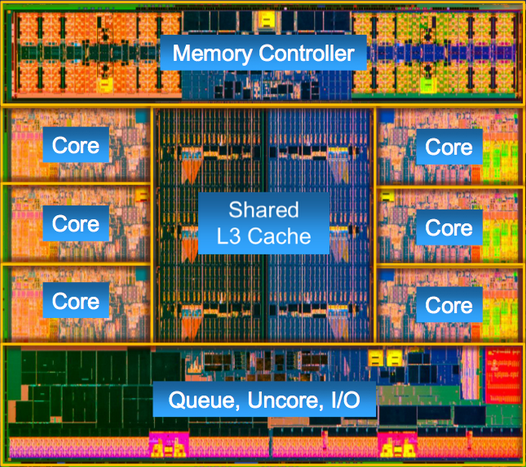
\includegraphics[width=0.5\textwidth]{esqProc}
    \caption{Schema of a typical 6 core processor}
    \label{fig:esqProc} %Establece una etiqueta para la figura
\end{wrapfigure}

In this thesis, what is has been done is to disable threads. Thanks to this processor architecture, the processor is divided in 6 hardware cores which are subdivided in 2 threads or logic cores. Figure \ref{fig:esqProc} represents the schema of the processor.

As the OS can manage the configuration of each thread separately, the main objective has been to disable them in order to understand how the number of threads is related to the performance of the server. Disabling threads leads to two reactions: the power consumption decreases, but it also decreases the performance of the cpu. Disabling threads will only reduce the performance because disabling is just not allowing a process to be executed by this processor.

The idea is that by disabling threads we can analyze if the time a benchmark elapse grows and if it increases the energy consumed by the benchmark. 

\subsubsection{chcpu}

To carry out this undertaking it has been used chcpu which is a command part of the util-linux package. Chcpu can modify the state of CPUs. It can enable or disable CPUs, scan for new CPUs, change the CPU dispatching mode of the underlying hyper-visor, and request CPUs from the hyper-visor (configure) or return CPUs to the hyper-visor (deconfigure).

In this case, only the function of disabling and enabling cpus has been used.

\begin{lstlisting}[language=Bash]
chcpu disable <Core number [1...11]>
\end{lstlisting}

Notice that core 0 cannot be disabled because it is the master core where the OS runs.

In the next chapter, the analysis about this actuation technique will be detailed.

\subsection{Off-lining Memories}

The main goal of this technique is to off-line memory modules seeking for a power consumption reduction.

In the last memory hotplug update, there is a folder structure used to see and change the status of the memory blocks. There are three important files in the hot-plug/hot-off-lining process:


\begin{tabular}{ p{2.4cm} p{10.5cm}}
  \bf State & When reading, it contains the online/offline state and when writing, it allows to change between online, offline, online kernel $-$ At the same time this memory block is online , it is configured as kernelcore $-$ and online movable $-$ At the same time this memory block is online, it is configured as movablecore \\ \\
  \bf Removable &  Indicates if the memory block is removable or not. It contains an 1 if is removable and a 0 if it is not \\ \\
  \bf Valid\_zones &Specifics the states the memory block can switch to\\
\end{tabular}


As we will just explain how removing memories work, we will talk about Hot-Remove instead of Hot-plug. In order to properly switch off a DIMM, there are three phases in Memory Hot-Remove:

\begin{description}
 \item[Step 1] Movable Memory Set
 \item[Step 2] Logical Memory Remove
 \item[Step 3] Physical Memory Remove. (To be developed)
\end{description}

\subsubsection{Movable Memory Set}

This phase intends to make the whole memory block be unused. The problem is that memory offline can fail if the memory block includes memory which cannot be freed. Memory that can be freed is that whose all pages can be migrated to other memory block.

To understand how memory permissions work, we need to explain all memory migratable configurations. Memory modules can be configured as kernelcore, movablecore and not-configured.

\begin{itemize}
    \item[$-$] Parts of the memory that are configured as \emph{kernelcore} are reserved for processes of the kernel only. These pages cannot be moved, so this parts cannot be migratable and, in short, removed.
    \item[$-$] Parts of the memory that are configured as \emph{movablecore} are reserved for processes that can be reallocated in other memory modules. This is the amount of memory we can be sure we will be able to logically remove.
    \item[$-$] Finally, the memory does not have to be configured.
\end{itemize}

This configuration must be made through a booting option of the kernel in the GRUB stage.
\subsubsection{Actuation technique: GRUB}

GNU GRUB is a boot loader package from the GNU Project, which allows a user the choice to boot one of the multiple operating systems installed on a computer or select a specific kernel configuration available on a particular operating system's partitions.

So, when grub starts, a movablecore or kernelcore has to be set in order to select the amount of memory wanted to be migratable and not-migratable.

To test if this can be modified, we followed the next instructions:

\begin{lstlisting}[language=Bash]
#When grub starts, press "e" to enter in GRUB configuration.
#Add the memory option at the end of the following line:

linux /boot/vmlinuz-linux <More boot options>

#Finally, press "b" to boot with the new parameters.
\end{lstlisting}

This only makes changes for this time, if the changes must be permanent, this file has to be modified:

\begin{lstlisting}[language=Bash]
# In file /etc/default/grub add
# one or both of the following lines:

KERNELCORE = <Amount of memory in GB>
MOVABLECORE = <Amount of memory in GB>

#Finally, execute:

grub-mkconfig -o /boot/grub/grub.cfg

\end{lstlisting}



The problem is that when the OS starts, there is no information about which memory belongs to movable or to not movable.

\subsubsection{Logical Memory Remove}

In the second step, using the sysfs interface just have to change the "state" file to offline and if the first step was correctly completed, this step must be ok.

When a memory is logically removed, no task can allocate information in this memory block until it is plugged again. At first, there is no sign that just logical remove saves power. The technique saves power if when a memory is off-lined, power is saved.

It is expected that physical memory remove will save energy when it is implemented.

\subsubsection{Conclusion}

During this thesis, several attempts of hot-removing memories has been made. Despite, it is not possible to reduce the power consumption generated by the memories.

Thanks to this work, some gaps have been identified in this issue. First of all, memories hot removing is not completely implemented at this moment. There is a lot of work pending to be done.

The server that the group has in its facilities does not have the latest version of centOS. Actually, it has the CentOS release 6.6 (Final). CentOS is currently in version 7.0. With this 6.6 version, configuration files are not the definitely ones and logical memories remove cannot be properly done.

Hopefully, some personal computers in the group has CentOS 7.0 installed. Using this computers, memories could be logically removed, but not physically removed. The issue comes from that memories can be disabled and the SO is notified of it, but then there is no way to know which physical module corresponds to the logical module, so the SO cannot turn it off.

\subsection{Changing fan speed}

Changing Fans Speed was one of the first goals of this thesis due to previous work showed that this could be a technique that could easily reduce a great amount of power consumption.

Despite the other subsystems are directly connected to the Baseboard Management Controller, fans are controlled by the Service Processor. \cite{serverSpecif}

The service processor is a separate, dedicated internal processor located on the motherboard of the server. It operates independently from the server’s CPU and operating system (OS), even if the CPU or OS is locked up or otherwise inaccessible.
%http://www.emersonnetworkpower.com/en-US/Latest-Thinking/Pages/avocent-thought-leadership-service-processor-management.aspx

The service processor monitors the server’s on-board instrumentation (temperature sensors, CPU status, fan speed, voltages), provides remote reset or power-cycle capabilities, enablse remote access to basic input/output system (BIOS) configuration or OS console information and is responsible for the fan speed control.

The difficulty of this task comes from the fact that the server uses a Service Processor to control the fan speed. Common \emph{Linux} speed control scripts modifies only the fan speed if it is controlled through the BMC, for this reason, they are not useful for this thesis.

The service processor uses an IPMI technology. For this reason, in this thesis is used ipmitool as the tool to control the service processor.

Ipmitool lets you manage Intelligent Platform Management Interface (IPMI) \cite{ipmiSpec} functions of either the local system, via a kernel device driver, or a remote system, using IPMI V1.5 and IPMI v2.0. In this case, it is used IPMI v2.0
%Enlace a las especificaciones de ipmi v2

The next step was to be able to change the speed through the \emph{BIOS}. BIOS have direct communication with the SP an is able to change the fan speed. The issue is that there is only one option which is to add a threshold to the current fan speed, but not reducing the speed what was the aim of the thesis. Previous work of the GreenLSI has modeled the behaviour of the fan consumption depending on the air flow.

Now, before explaining the third step, it is important to distinguish between two ways of introducing improvements into the server: the less invasive, which consists in adding a new abstraction layer that enables us to do whatever we want without modifying what it was already there - it can be both hardware or software - and the intrusive one which is to modify something that is already in the code or in the hardware.

The third attempt was related to analyze the code of the \emph{kernel} of the SP to find out how the SP decides the fan speed. The idea was to modify the code to allow us to change the speed wherever we want in some way. Despite all the code is available, it was not clear where the decision algorithm was so it cannot be changed.

Finally, the single option is to change it through \emph{IPMI} which allows the BMC and the SP to give parameters and information to each other.

Using IPMI \cite{serverConfigIPMI}, there were two processes that could had helped us in this task:

\begin{itemize}
    \item[$-$] Giving some raw commands:
\end{itemize}

This was the first idea of how to modify the fan speed using IPMI. There is a document that describes Facebook's Fan Speed Control (FSC) and its update methodology
The aim Facebook has writing this document is to standardize how the server management controller manages FSC parameters.

With this new commands, two points can be managed through ipmi. On the one hand, Pulse Width Modulation (PWM) can be set directly. To perform this feature, a raw command of this layout must be sent: 

\begin{lstlisting}[language=Bash]
impitool [options] raw 0x30 <PWM ID> <PWM value> 
            #0x30 allows us to send FSC commands.
\end{lstlisting}

On the other hand, Facebook provides some simple control or information algorithms that can be set as profile of the fans in order to control the fan speed or calculate related parameters. There are four algorithms divided into Linear and Non-Linear.

\begin{itemize}
    \item[$*$] \textbf{Linear. Temperature: }This set controls the fans speed depending of the temperature. If it exceeds a threshold value, fan speed increases. The algorithm outputs the pwm value in percentage.
    \item[$*$] \textbf{Linear. FAN RPM: }This set controls the average of Cubic Feet per Minute (CFM) that the fans move. As input it has the Fan rpm and outputs the CFM.
    \item[$*$] \textbf{Linear. Power: }This set calculates the relation between the power used by the fans and the PWM in which it is translated.
     \item[$*$] \textbf{Non-Linear. PID Controller: }PID is the acronymus of Proportional, Integral, Derivative (PID) controller which is a widely used control loop feedback mechanism. This is a non-linear algorithm that allows to control fan speed control. It is more complex than the others to be more exact.
\end{itemize}

To change this profiles, entering and exiting in update mode is required to the changes take effect.

Despite it is well documented by the specification of the Facebook's Decathlete server, it is not well implemented in the S2600GZ server from Intel, which is supposed to fulfill the Decathlet's specifications. That is why it cannot be tested in this thesis.

\begin{itemize}
    \item[$-$] Changing the threshold parameter
\end{itemize}

Finally, another way of changing the fan speed was tested. The SP uses several registers to determine if the temperature of the server is within the correct values or, by contrast, it is over the well-functioning range. The idea was to change this registers in order to make the server run the fans slower to see how the temperature and the performance changes.

\begin{lstlisting}[language=Bash]
ipmitool sensor thresh <sensor name> lower <lower 
    non-recovery value> <lower critical value> <lower
    non-critical value>

ipmitool sensor thresh <sensor name> upper <upper
    non-critical value> <upper critical value> <upper
    non-recovery value>
\end{lstlisting}

Seemingly, it is not well implemented. When one of this registers is changed, all the fans began to run at the maximum speed, 12 000 RPM and never reduce their speed despite there is no issue. We leave for future the debugging of this technique.

\subsubsection{Conclusion}

%Muy interesante esta página http://www.opencompute.org/wiki/Server/SpecsAndDesigns
As it is described in the document of the OCP \cite{fanspeed}, the Open Compute Project defined a new algorithm to manage fan speed of the servers. The 0.1 version of this algorithm was published in 2014. The problem is that a document from the OCP does not automatically generates a new release of the Intel Service Processor.

% Creo que es este firmware https://downloadcenter.intel.com/download/24617/Intel-Server-Board-S2600GZ-GL-Firmware-Update-for-IDA-and-OFU
In this case, the problem is similar to what occurs with memories hotplug. The version of the SP's kernel is not the latest one and it cannot be checked if the latest version has already implemented the algorithm published in the paper. To update to the latest version and to check if it works properly is to be done.


\subsection{Summary}

To sum up, here is a table with the studied levels for each subsystem. It is important to emphasise that the aim has been always to find a higher level solution.


\begin{table}[H]
\centering
\label{my-label}
\begin{tabular}{c|cccc}
LEVEL & MEMORIES & CPU Disabling & DVFS & FAN SPEED\\ %\cline{2-5}
\hline \\
User Space & \multirow{3}{*}{YES} & Implemented & Implemented & NO \\ \\
Kernel  &                   &  &  & NO \\ \\
BIOS &      Limited             &  &  & Offset only \\ \\
SP &                   &  &  & Firmware dependant \\ 
\end{tabular}
\caption{Summary of the possible actuation levels over Intel S2600GZ}
\end{table}

In memories subsystem, the solution is a combination of User-space and kernel levels.



